\section*{Содержание работы}
\textit{Цель работы}: построение гистограммы и эмпирической функции распределения.
\begin{enumerate}[wide=0pt]
	\item Для выборки объема n из генеральной совокупности X реализовать в виде программы на ЭВМ:
	\begin{enumerate}
		\item вычисление максимального значения $M_{max}$ и минимального значения $M_{min}$;
		\item размаха $R$ выборки;
		\item вычисление оценок $\hat{\mu}$ и $S^2$ математического ожидания MX и дисперсии DX;
		\item группировку значений выборки в $m = [\log_2n] + 2$ интервала;
		\item построение на одной координатной плоскости гистограммы и графика функции плотности распределения вероятностей нормальной случайной величины с математическим ожиданием $\hat{\mu}$ и дисперсией $S^2$;
		\item построение на другой координатной плоскости графика эмпирической функции распределения и функции распределения нормальной случайной величины с математическим ожиданием $\hat{\mu}$ и дисперсией $S^2$.
	\end{enumerate}
	\item Провести вычисления и построить графики для выборки из индивидуального варианта.
\end{enumerate}

\section*{Теоретические сведения}

Множество возможных значений случайной величины $X$ называют \textbf{генеральной совокупностью} 
случайной величины $X$.

Любое возможное значение $\vec{x} = (x_1, \dots x_n)$ случайной выборки $\vec{X}_{n}$ будем называть \textbf{выборкой} из генеральной совокупности $X$. Число n характеризует объем выборки, а числа $x_i$ представляют собой элементы выборки $\vec{X}_{n}$.

Пусть $\vec{x} = (x_1, \dots x_n)$ — выборка объема $n$ из генеральной совокупности $X$. 
Ее можно упорядочить, расположив значения в неубывающем порядке:

\begin{equation}
x_{(1)} \leq x_{(2)} \leq x_{(3)} \leq \dots \leq x_{(n)}
\end{equation}


Такую последовательность чисел из формулы 1 называют \textbf{вариационным рядом}.

Тогда $x_{(1)}$ является \textbf{минимальным} значением выборки, а $x_{(n)}$ - \textbf{максимальным} значением выборки.

\textbf{Размахом} выборки называют разность между максимальным и минимальным значениями.

Рассмотрим функцию $n(x, \vec{X_n})$, которая для каждого значения $x \in R$ и каждой реализации $\vec{x_{n}}$ случайной выборки $\vec{X}_{n}$ принимает значение $n(x, \vec{x_n})$, равное числу элементов в выборке $\vec{x_n}$, меньших x.

Тогда \textbf{эмпирической функцией распределения} называется функция:
\begin{equation}
F(x, \vec{X_n}) = \frac{n(x, \vec{x_n})}{n}
\end{equation}

Оценку математического ожидания можно подсчитать по формуле:
\begin{equation}
\hat{\mu}(\vec{X}) = \cfrac{1}{n}\sum_{i = 1}^{n}x_i,
\end{equation}
Смещённую выборочную дисперсию можно подсчитать по формуле:
\begin{equation}
S_{n}^2(\vec{X}) = \cfrac{1}{n}\sum_{i = 1}^{n}(x_i - \bar{x})^2.
\end{equation}
Исправленную выборочную дисперсию можно подсчитать по формуле:
\begin{equation}
S^2(\vec{X}) = \cfrac{1}{n - 1}\sum_{i = 1}^{n}(x_i - \bar{x})^2.
\end{equation}


При больших объемах выборки $n$ обычно производят группирование исходных данных следующим образом. 
Промежуток $J = [x_{(1)} , x_{(n)}]$, содержащий все выборочные значения, разбивают на $m$ 
полуинтервалов $J_1, \dots , J_m$ , как правило, одинаковой длины $\delta$ и таких, 
что каждый из них, кроме последнего, содержит левую границу, 
а последний содержит обе границы, и подсчитывают число $n_i$ элементов выборки, 
попавших в i-ый промежуток $J_i$, а результаты представляют в виде таблицы, 
которую называют \textbf{интервальным статистическим рядом}.

\textbf{Эмпирической плотностью} распределения соответствующей выборке $\vec{x}$ называется функция:
\begin{equation}
f_n(x) = 
\begin{cases}
\cfrac{n_i}{n \cdot \Delta} & ,x \in J_i, \\
0 & ,\text{иначе.}
\end{cases}
\end{equation}
График эмпирической функции плотности называется \textbf{гистограммой}.

Пусть на выборке $\vec{x}$ определён интервальный статистический ряд. Эмпирической функцией распределения интервального ряда называется функция:
\begin{equation}
F(J_i) = \frac{1}{n}\sum_{j = 1}^{i}J_i
\end{equation}

\newpage
\section*{Код программы}
На листинге 1 представлен код программы:
\FloatBarrier
\begin{lstinputlisting}{src/main.m}
\end{lstinputlisting}
\FloatBarrier

\section*{Результаты работы программы}
На рисунке 1 представлен график гистограммы и графика функции плотности распределения вероятностей нормальной случайной величины:
\FloatBarrier
\begin{figure}[h]
	\begin{center}
		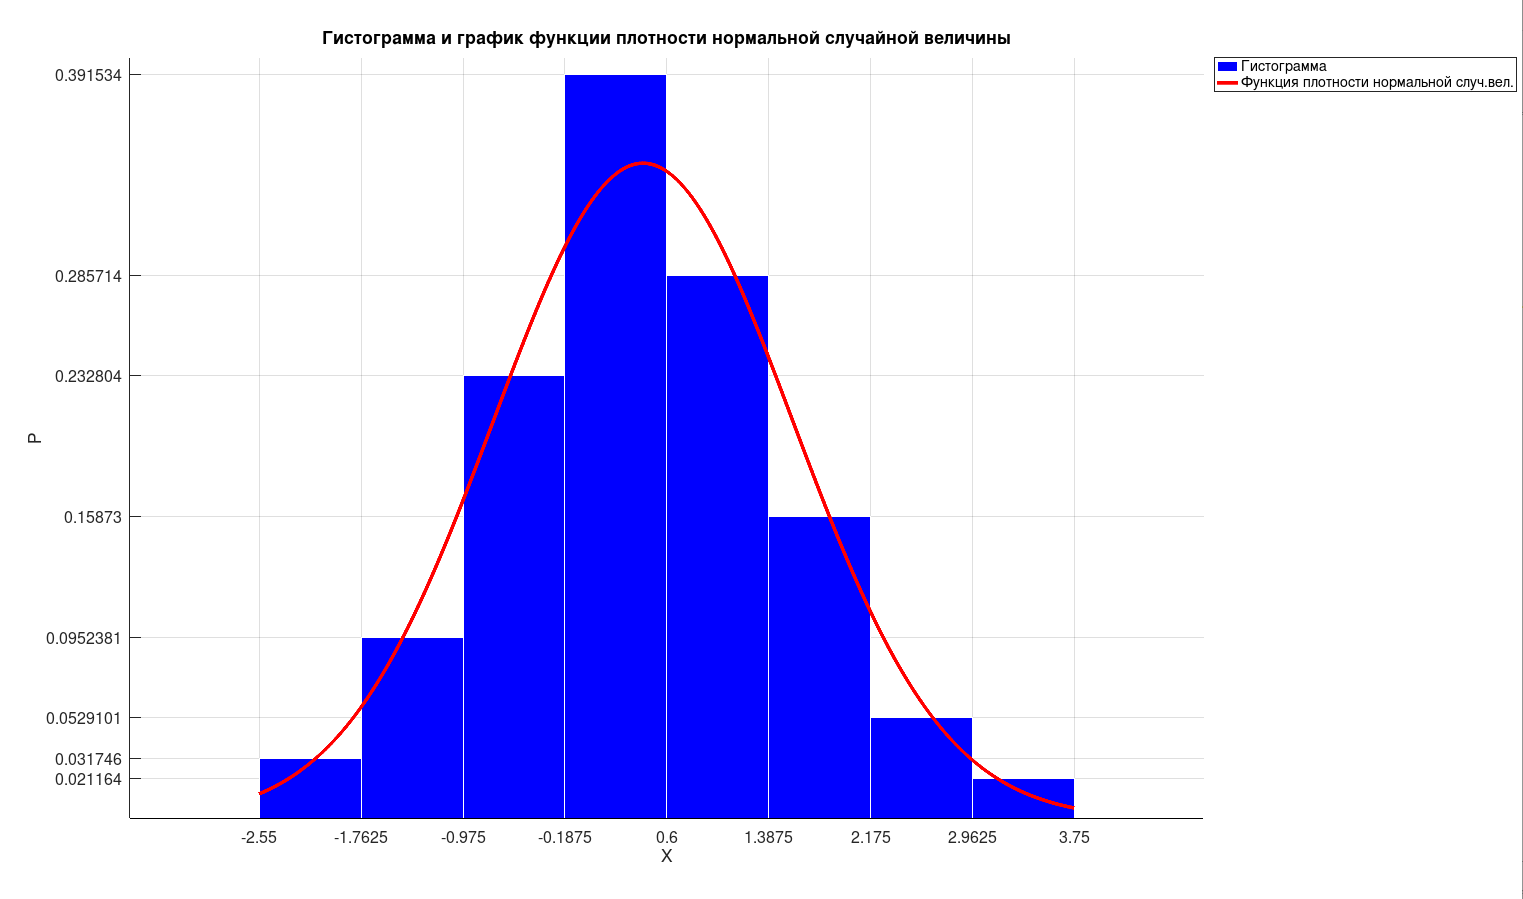
\includegraphics[width=\linewidth, height=10cm]{inc/hist.png}
	\end{center}
\end{figure}
\FloatBarrier

На рисунке 2 представлен  графика эмпирической функции распределения и функции распределения нормальной случайной величины:
\FloatBarrier
\begin{figure}[h]
	\begin{center}
		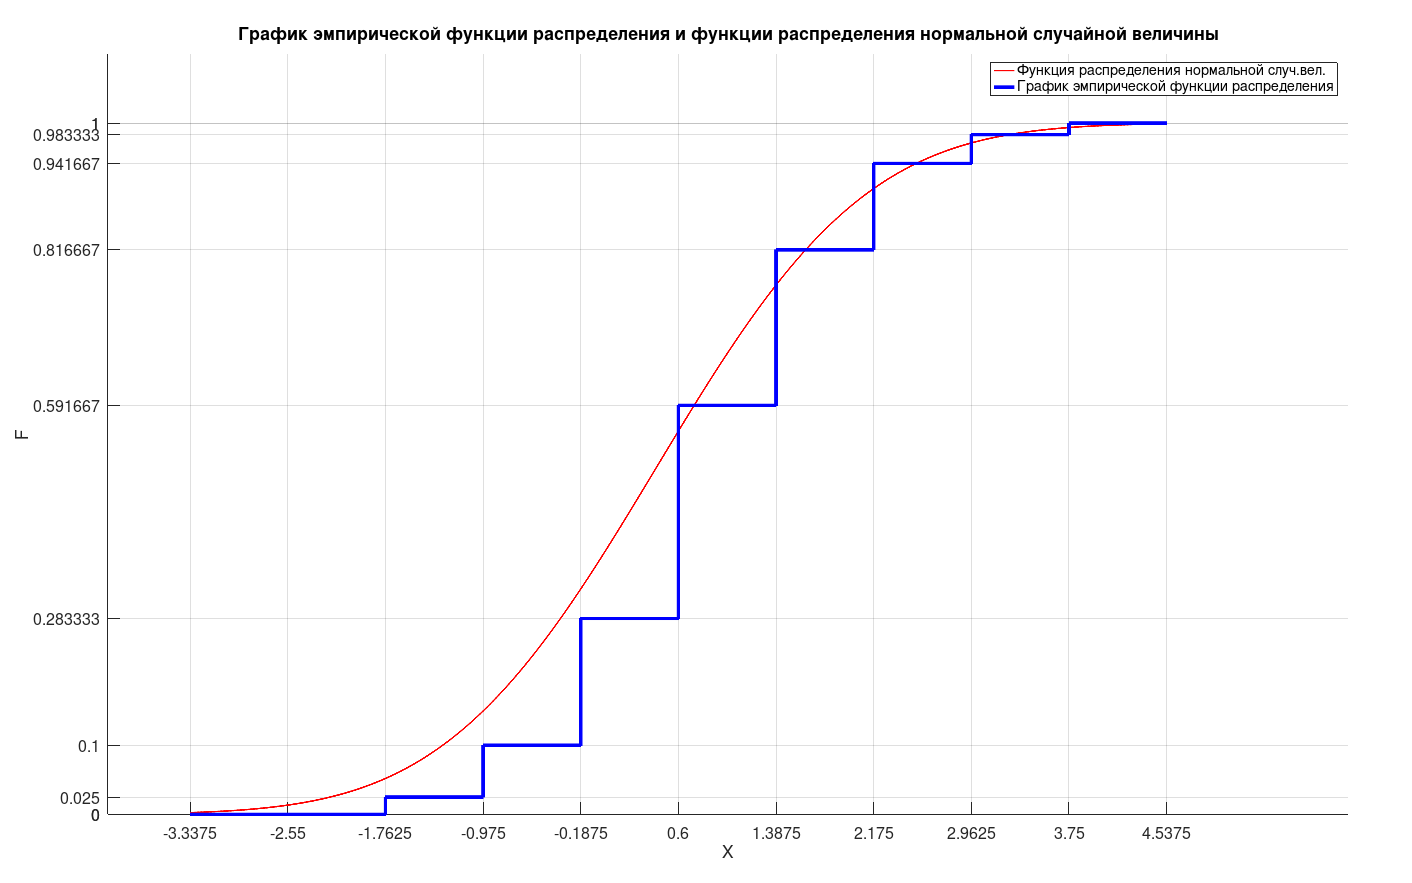
\includegraphics[width=\linewidth, height=10cm]{inc/cdf.png}
	\end{center}
\end{figure}
\FloatBarrier

Результат работы программы представлен на рисунке 3:
\FloatBarrier
\begin{figure}[h]
	\begin{center}
		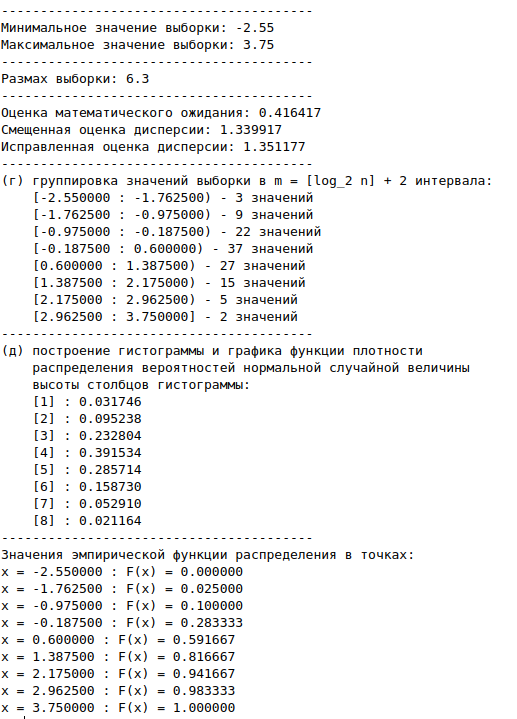
\includegraphics[width=\linewidth]{inc/result.png}
	\end{center}
\end{figure}
\FloatBarrier

